\section{Convex Approximation of Contact Dynamics}
\label{sec:convex_approximation}

Previous work from Anitescu \cite{bib:anitescu2006} introduces an approximation
of the nonpenetration constraint Eq. \eqref{eq:scheme_nonpenetration} that
together with Eqs. \eqref{eq:scheme_mdp_multiplier}-\eqref{eq:scheme_mdp_cone}
leads to a convex formulation in impulses. Though not strictly applicable to
contact problems, later on Todorov \cite{bib:todorov2011, bib:todorov2014} uses
the \emph{Gauss's principle of least constraint} to obtain a regularized form of
Anitescu's formulation that admits a unique solution. Moreover, Todorov shows
that impulses can be constructed from the computed velocities, an operation
referred to as \textit{analytical inverse dynamics}.

In this section we build from this previous work to write a convex formulation
of compliant contact. Our convex optimization problem is formulated in terms of
velocities and we show that (with symplectic Euler) its dual corresponds to
Todorov's \cite{bib:todorov2014} formulation in impulses. Further, we use
Todorov's \textit{analytical inverse dynamics} to eliminate constraints
analytically and write an unconstrained formulation.


\section{A Primal Formulation of Compliant Contact}

In this section we augment the balance of momentum stated in Eq.
(\ref{eq:momentum_linearized}) so that contact impulses model Colulomb friction
and satisfy the principle of maximum dissipation when sliding. 

An alternative is to use a convex approximation as stated in Eq.
(\ref{eq:dual_cost}). However, this formulation is severely ill conditioned due
to the fact that contact forces for rigid body dynamics problems are most often
underdetermined. Even if compliance is added in the normal direction, friction
forces for the simplest problem configurations will be underdetermined.
Regularization in Eq. (\ref{eq:dual_regularized}) helps to solve this problem in
theory but it leads to very ill conditioned systems of equations in practice. 

We make the following observation for the convex approximation in Eq.
(\ref{eq:dual_cost}); even if the set of contact forces is not unique (when no
regularization is added), velocities are. This fact inspired the search
for an equivalent formulation but in velocities instead of impulses. Such a
\textit{primal} formulation is presented in \cite{bib:mazhar2014} for rigid
contact, though to the knowledge of the authors a practical solver based on this
formulation has never been presented.

In this section we extend the formulation in \cite{bib:mazhar2014} to include
the modeling of compliance and in Sections
\ref{sec:unconstrained_convex_formulation} and \ref{sec:solver_details} we
describe a methodology to solve it in practice.

We write our primal formulation of compliant contact by introducing a new
decision variable $\vf{\sigma}\in\mathbb{R}^{3n_c}$ as
\begin{equation}
	\begin{aligned}
	\min_{\mf{v},\bsigma} \quad & \ell_p(\mf{v},\bsigma) = \frac{1}{2}(\mf{v}-\mf{v}^*)^T\mf{A}(\mf{v}-\mf{v}^*) + \frac{1}{2} \Vert\bsigma\Vert_{R}^2\\
	\textrm{s.t.} \quad & \mf{g} = (\mf{J}\mf{v}-\hat{\mf{v}} + \mf{R}\bsigma) \in \mathcal{F}^*\\
	\end{aligned}
	\label{eq:primal_regularized}
\end{equation}
where $\mathcal{F^*}=\prod_{k=1}^{n_k}\mathcal{F}^*_k$ is the dual of the convex
set $\mathcal{F}$. The positive diagonal matrix $\mf{R}\in\mathbb{R}^{3n_c\times
3n_c}$ and the vector of stabilization velocities $\hat{\mf{v}}$ encode the
problem data needed to model compliant contact. We will establish a very clear
physical meaning for these terms when we provide analytical expressions for the
impulses in Section \ref{sec:analytical_inverse_dynamics}. Finally,
$\Vert\bsigma\Vert_R^2=\bsigma^T\mf{R}\bsigma$.

\RedHighlight{Per Frank's request. The fact that \ref{eq:primal_regularized},
\ref{eq:dual_regularized} and \ref{eq:primal_unconstrained} are equivalent is
very important. State that as a theorem even if the proof is simple.}

\RedHighlight{Frank: You should say then that (v, sigma) is primal optimal and
gamma is dual optimal, and then give the explicit formulae, pointing out that
sigma = gamma.}

The Lagrangian of the primal formulation in Eq. (\ref{eq:primal_regularized}) is
\begin{equation}
	\mathcal{L}(\mf{v},\bsigma,\vf{\gamma}) = \frac{1}{2}(\mf{v}-\mf{v}^*)^T\mf{A}(\mf{v}-\mf{v}^*) + \frac{1}{2} \Vert\bsigma\Vert_{R}^2 - \vf{\gamma}^T\mf{g}
	\label{eq:primal_lagrangian}
\end{equation}
with $\vf{\gamma}\in\mathcal{C}$ the dual variable to enforce the constraint
$\vf{g}\in \mathcal{C}^*$. We can obtain the dual of Eq.
(\ref{eq:primal_regularized}) by minimizing the Lagrangian jointly in the
variables $\mf{v}$ and $\bsigma$ and replacing the result back to obtain the
dual cost $\ell_d(\vf{\gamma})$. Minimizing jointly in the variables $\mf{v}$
and $\bsigma$ leads to the conditions
\begin{eqnarray}
	\mf{A}(\mf{v}-\mf{v}^*) &=& \mf{J}^T\vf{\gamma}\\
	\vf{\sigma} &=& \vf{\gamma}
\end{eqnarray}
where with the first equation we find out that multipliers $\bgamma$ are indeed
impulses and we recover the balance of momentum, and the second equation allows
us to eliminate $\vf{\sigma}$. When we replace these results back into the
Lagrangian in Eq. (\ref{eq:primal_lagrangian}) we obtain the dual
\begin{eqnarray}
	\min_{\gamma\in \mathcal{C}} \ell(\bgamma) =
	\frac{1}{2}\bgamma^T(\mathbf{W}+\mathbf{R})\bgamma + {\bm r}^T
	\bgamma
\end{eqnarray}
where, in contrast to Eq. (\ref{eq:dual_regularized}), the Delassus operator
$\mf{W}=\mf{J}\mf{A}\mf{J}^T$ now also contains the contribution of internal
force elements and $\mf{r}=\mf{v}_c^*-\hat{\mf{v}}$.

\section{Analytical Inverse Dynamics}
\label{sec:analytical_inverse_dynamics}

Given a set of $n_k$ constraints defined by their constraint velocity
$\vf{v}_{c,k}$ and impulse $\bgamma_k\in\mathcal{C}_k$, we form a global vector
$\vf{v}_c$ that concatenates all constraint velocities and define the Cartesian
product $\mathcal{C}=\prod_{k=1}^{n_k}\mathcal{C}_k$. Since each $\mathcal{C}_k$
is convex, so is $\mathcal{C}$. We proceed in a similar way with $\bgamma_k$,
$\hat{\vf{v}}_k$, $\mf{R}_k$, $\mf{J}_k$ to obtain the global quantities
$\bgamma$, $\hat{\mf{v}}$, $\mf{R}$, $\mf{J}$. With these definitions we can
compactly write the constraint $\bgamma\in\mathcal{C}$ for all impulses in the
problem.


\section{An Unconstrained Convex Formulation}
\label{sec:unconstrained_convex_formulation}

The primal formulation in Eq. (\ref{eq:primal_regularized}) and its dual in Eq.
(\ref{eq:dual_regularized}) are equivalent. Since both are strictly convex, they
share the same unique solution. In particular, they both share the same
analytical inverse dynamics solution described in Section
\ref{sec:constraints_based_modeling_framework}.

Recall from Section \ref{sec:constraints_based_modeling_framework} that the
inverse dynamics solution provides the impulse as a function of the constraint
velocity as
\begin{eqnarray}
	\bgamma(\mf{v}_c) = P_\mathcal{C}(\mf{y}(\mf{v}_c))
\end{eqnarray}
where $\mf{y}(\mf{v}_c) = -\mf{R}^{-1}(\mf{v}_c-\hat{\mf{v}})$ and we have
analytical algebraic expressions for the projection $P_\mathcal{C}(\mf{y})$.

This allow us then to substitute $\bsigma=\bgamma=P_\mathcal{C}(\mf{y})$
into Eq. (\ref{eq:primal_regularized}) to obtain an unconstrained convex
optimization problem in the velocities only
\begin{eqnarray}
	\min_{\mf{v}} \ell_p(\mf{v}) =
	\frac{1}{2}(\mf{v}-\mf{v}^*)^T\mf{A}(\mf{v}-\mf{v}^*) +
	\ell_R(\mf{y}(\mf{v}))
	\label{eq:primal_unconstrained}
\end{eqnarray}
with the regularizer
\begin{equation}
	\ell_R(\mf{y}(\mf{v})) = \frac{1}{2}\Vert P_\mathcal{C}(\mf{y}(\mf{v}))\Vert_R^2
\end{equation}

Though this problem is strictly convex and can be solved using Newton's method
we make the following observations
\begin{enumerate}
	\item Since projections $P_\mathcal{C}$ are piecewise continuous, the cost
	$\ell_p$ is piecewise continuous.
	\item The Hessian $\mf{H}=\nabla^2\ell_p$ is not continuous, with large
	variations of \textit{curvature}. While this is not a problem for Newton's
	method given its \textit{affine invariance} property in theory, in practice
	we will use an analytically computed Hessian to avoid numerical round-off
	errors.
	\item\label{item:line_sarch} Since the problem is strictly convex, line
	search combined with Newton's method leads to guaranteed convergence.
	However, given the piecewise nature of $\ell_p$ and its large variations in
	curvature, in practice we find we need a specially designed line search to
	preserve accuracy.
\end{enumerate}

Item \ref{item:line_sarch} is of utmost important in practice. We'll show a
strategy that allows to perform line search with machine epsilon precision. A
careful pre-computation of commonly occurring terms enable us to perform this
step for a small computation cost when compared to Hessian assembly and
factorization. While machine epsilon accuracy is not required in practice, we
show that the cost to achieve this level of convergence is negligible and it is
well worth it for a robust implementation that can handle very stiff systems
(with small regularization).

In the next subsection we show how to compute the required gradients for
Newton's method and, as a consequence, we verify the strict convexity of
$\ell_p$.


\subsection{Gradients}
\label{sec:gradients}

In this section we summarize the main results required for implementation.
Detailed derivations are provide in the Appendix \ref{app:gradients_derivation}.
We will see that in order to compute both the gradient and Hessian of the cost
we only need analytical expressions of the projection $P_\mathcal{C}$ and its
gradient.

The gradient of the primal cost $\ell_p$ is
\begin{equation}
	\nabla_\mf{v}\ell_p(\mf{v}) = \mf{A}(\mf{v}-\mf{v}^*) + \nabla_\mf{v}\ell_R
\end{equation}

Computing this gradient might seem a daunting enterprise, but after substitution
of $\nabla_\mf{v}P_\mathcal{C}$ the result is beautifully simple
\begin{equation}
	\nabla_\mf{v}\ell_p(\mf{v}) = \mf{A}(\mf{v}-\mf{v}^*) - \mf{J}^T\bgamma
	\label{eq:primal_gradient}
\end{equation}

Which recovers the momentum balance since Newton's method solves for
$\nabla_\mf{v}\ell_p=\mf{0}$.

Instead of directly computing the Hessian $\nabla_\mf{v}^2\ell_R$ (which would
lead to exactly the same result), we can instead compute $\nabla_\mf{v}^2\ell_p$
by taking the gradient of Eq. (\ref{eq:primal_gradient}). The result is
\begin{eqnarray}
	\nabla_\mf{v}^2\ell_R(\mf{v}) &=&
	\mf{J}^T\nabla_{\mf{v}_c}\!\bgamma\,\mf{J}\nonumber\\
	\nabla_{\mf{v}_c}\bgamma &=& -\nabla_\mf{y}\bgamma \mf{R}^{-1}
	\label{eq:ellR_hessian}
\end{eqnarray}
where $\nabla_{\mf{v}_c}\!\bgamma$ is a block diagonal matrix where each
diagonal elements is the $n_k\times n_k$ matrix
$\nabla_{\mf{v}_{c,k}}\!\bgamma_k$ for the $k\text{-th}$ constraint. As shown in
Appendix \ref{app:gradients_derivation}, $\nabla_{\mf{v}_c}\bgamma\succeq 0$ and
thus $\nabla_\mf{v}^2\ell_R(\mf{v})\succeq 0$.

Finally, the Hessian needed in Newtons's method is
\begin{equation}
	\mf{H}= \nabla_\mf{v}^2\ell_p(\mf{v}) = \mf{A} -\mf{J}^T\nabla_\mf{y}\bgamma \mf{R}^{-1}\mf{J}	
	\label{eq:ell_hessian}
\end{equation}
which, since $A\succ 0$, is strictly positive definite. We note however that
showing $\nabla_\mf{v}^2\ell_p(\mf{v})\succ 0$ is not enough for $\ell_p$ to be
strictly convex. Since $\ell_p$ is a piecewise function, we must additionally
require that the directional derivative across the boundary
$\partial\mathcal{C}$, of $\mathcal{C}$ increases. Formally, if $\mf{\nu}$ is
the normal to $\partial\mathcal{C}$, then we require
\begin{equation}
	\frac{\partial \ell_p^-}{\partial \nu} \le \frac{\partial \ell_p^+}{\partial \nu}
\end{equation}
we show this to be the case in Appendix \ref{app:gradients_derivation} which
then leads to the confirmation that $\mf{H}\succ 0$.


\section{Assembling Equality Constraints}
\label{sec:assembling_equality_constraints}
\todo{Write how to the Hessian for equality constraints is constant and can be pre-computed.}

% Dummy comment so that files shows up in Reviewable.

\textit{Inverse dynamics} refers to the computation of the impulses given known
velocities of the system. It is shown in \cite{bib:todorov2014} that contact
impulses are solution to the convex program stated in Eq.
(\ref{eq:y_projection}). This problem can be solved analytically using simple
geometry. By noticing that the change of variables
$\tilde\bgamma=\vf{R}^{1/2}\bgamma$ (and respectively
$\tilde{\vf{y}}=\vf{R}^{1/2}\vf{y}$) leads to a projection with Euclidian norm
on a cone $\mathcal{F}_{\tilde\mu}$ with friction coefficient
$\tilde\mu=\mu\,(R_t/R_n)^{1/2}$
\begin{eqnarray}
	P_\mathcal{F_{\tilde\mu}}(\tilde{\vf{y}})&=&\argmin_{\tilde\bgamma\in\mathcal{F_{\tilde\mu}}}
		\quad \frac{1}{2}\Vert\tilde\bgamma-\tilde{\vf{y}}\Vert_2^2\nonumber\\
	P_\mathcal{F}(\vf{y}) &=&
	\vf{R}^{-1/2}P_\mathcal{F_{\tilde\mu}}(\tilde{\vf{y}})
	\label{eq:local_optimization_problem_tilde}
\end{eqnarray}

The optimization problem in the Euclidean norm given by Eq.
(\ref{eq:local_optimization_problem_tilde}) can be solved by inspection. If
$\tilde{\vf{y}}\in\mathcal{F}_{\tilde\mu}$, then we simply have $\tilde{\bgamma}
= \tilde{\vf{y}}$, we call this \textit{Region I}. If however $\tilde{\vf{y}}$
is inside the polar cone $\mathcal{F}_{\tilde\mu}^\circ$, the closest point to
$\tilde{\vf{y}}_i$ within the (tilde) friction cone is zero, i.e.
$\tilde{\bgamma} =\vf{0}$. We call this \textit{Region III}. Finally, if
$\tilde{\vf{y}}$ is in the region outside both $\mathcal{F}_{\tilde\mu}$ and its
polar $\mathcal{F}_{\tilde\mu}^\circ$, then the closest point is it's Euclidian
projection on the boundary of $\mathcal{F}_{\tilde\mu}$. We call this
\textit{Region II}. Figure \ref{fig:cone_regions} shows a schematic of
$\mathcal{F}_{\tilde\mu}$, $\mathcal{F}_{\tilde\mu}^\circ$ and labels the three
different regions. From Fig. \ref{fig:cone_regions}, for a cone forming an angle
$\theta$ with the z axis, we have $\tan(\theta)=\tilde\mu$ and
$\cos(\theta)=1/(1+\tilde\mu^2)$. Then the projection of a point
$\tilde{\vf{y}}$ in Region II can be written as
\begin{eqnarray}
	\tilde{\bgamma}_t &=& \tilde{\mu}\tilde{\gamma}_n\hat{\vf{t}}\nonumber\\
	\tilde{\gamma}_n &=& \frac{1}{1+\tilde{\mu}^2}\left(\tilde{y}_n +
	\tilde{\mu}\tilde{y}_r\right)\nonumber		
\end{eqnarray}
where the tangent vector is defined as
$\hat{\vf{t}}=\vf{y}_t/\Vert\vf{y}_t\Vert=-\vf{v}_t/\Vert\vf{v}_t\Vert$. 
\begin{figure}[!h]
    \centering
    %\vspace{6pt}
    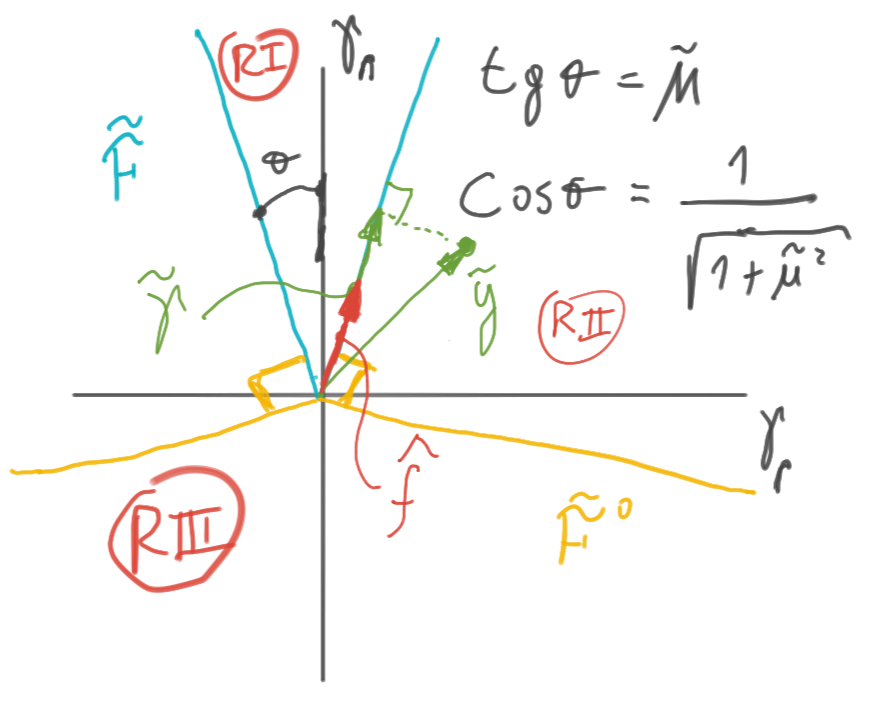
\includegraphics[width=0.45\columnwidth]{figures/cone_regions.png}
    \caption{Geometry of $\mathcal{F}_{\tilde\mu}$ and regions in the
    $\tilde{\vf{y}}$ space.}
    \label{fig:cone_regions}
\end{figure}

Finally, we obtain Eq. (\ref{eq:y_projection}) by applying the transformation
$\bgamma=\mf{R}^{-1/2}\tilde\bgamma$ to recover the impulses projected onto the
friction cone ${\mathcal{F}}_{\mu}$ using the norm in $\vf{R}$.

Though the tangent vector $\hat{\vf{t}}$ is not defined for $\vf{y}=\vf{0}$, the
projection still is, $P_\mathcal{F}(\vf{0})=\vf{0}$. In practice however, we
introduce a smooth \emph{soft-norm} defined as
$\|\vf{x}\|_s=\sqrt{\|\vf{x}\|^2+\varepsilon_s^2}$ and we define the tangent
vector as $\hat{\vf{t}}=\vf{y}_t/\Vert\vf{y}_t\Vert_s$. This newly defined tangent vector is smooth and has the desired property that it leads to the right
projection result in the limit to $\vf{y}\rightarrow 0$. In addition, not only
the projection is well defined, but also its gradients in Appendix
\ref{app:gradients_derivation}. In practice we use $\varepsilon_s=10^{-8}$.


\section{An Unconstrained Convex Formulation}
\label{sec:unconstrained_convex_formulation}

A remarkable property of the dual optimal solution, the impulses, is that they
can be can be constructed analytically from the optimal velocities of the primal
formulation in \eqref{eq:primal_regularized}. This is referred to as the
\textit{inverse dynamics} solution \cite{bib:todorov2014}. Moreover, given the
separable structure of the constraints, the impulse $\bgamma_i$ at the
$i\text{-th}$ contact point is the solution to the following convex optimization
problem
\begin{eqnarray}
	\bgamma_i(\vf{v}_{c,i})&=& P_{\mathcal{F}_i}(\vf{y}_i(\vf{v}_{c,i}))
	\nonumber\\
	&=&\begin{aligned} \argmin_{\bgamma\in\mathcal{F}_i} \quad &
		\frac{1}{2}(\bgamma-\vf{y}_i)^T\vf{R}_i(\bgamma-\vf{y}_i) \end{aligned}
	\label{eq:y_projection}\\
	\vf{y}_i(\vf{v}_{c,i}) &=& -\vf{R}_i^{-1}(\vf{v}_{c,i}-\hat{\vf{v}}_{c,i})	
\end{eqnarray}
where $\vf{R}_i\in\mathbb{R}^{3\times3}$ is the $k\text{-th}$ diagonal block of
the regularization matrix $\mf{R}$. That is, $\bgamma_i$ is the projection
$P_{\mathcal{F}_i}$ of $\vf{y}_i(\vf{v}_{c,i})$ onto the friction cone
$\mathcal{F}_i$ using the norm defined by $\vf{R}_i$.

We use the analytical inverse dynamics to write an unconstrained convex
formulation in terms of velocities only
\begin{eqnarray}
	\min_{\mf{v}} \ell_p(\mf{v}) = \frac{1}{2}\Vert\mf{v}-\mf{v}^*\Vert_{A}^2 +
	\frac{1}{2}\Vert P_\mathcal{F}(\mf{y}(\mf{v}))\Vert_R^2
	\label{eq:primal_unconstrained}
\end{eqnarray}
where, as with other quantities, we form $\mf{y}$ by stacking each
$\vf{y}_i$ from all contact pairs together. Given the separable structure of the
constraints, projection $P_{\mathcal{F}}(\mf{y})$ onto $\mathcal{F} :=
\mathcal{F}_1 \times F_2 \times \cdots \times \mathcal{F}_{n_c}$ in the norm
defined by $\mf{R}$ is formed by stacking together the individual projections
$P_{\mathcal{F}_i}(\vf{y}_i)$ from Eq. (\ref{eq:y_projection}).

The unconstrained formulation in Eq. (\ref{eq:primal_unconstrained}) includes
the same cost in velocities as the primal formulation from Eq.
(\ref{eq:primal_regularized}). However, the conic constraint $\mf{g}\in
\mathcal{F}^*$ in Eq. (\ref{eq:primal_regularized}) has been replaced by a cost
term using the analytical inverse dynamics. Lemma
\RedHighlight{Add proper reference} in Appendix \RedHighlight{Add proper reference} proofs
that the unconstrained cost $\ell_p(\mf{v})$ is strongly convex and
differentiable with Lipschitz continuous gradients. Therefore the problem
stated in Eq. (\ref{eq:primal_unconstrained}) has a unique solution.

We state the main result of this section in the following result, proved in
Appendix \ref{app:unconstrained_formulation_equivalance}.
\begin{theorem}
    The pair $\{\mf{v},\bsigma\}$, with velocities $\mf{v}$ solution to the
    unconstrained formulation in Eq. (\ref{eq:primal_unconstrained}) and
    $\bsigma=P_\mathcal{F}(\mf{y}(\mf{v}))$, is primal optimal of the primal
    formulation in Eq. (\ref{eq:primal_regularized}).
    \label{th:unconstrained_formulation_equivalance}
\end{theorem}

Section \ref{sec:sap_solver} presents our novel SAP solver specifically designed
to solve the unconstrained formulation in Eq. (\ref{eq:primal_unconstrained}).

